\begin{figure}[H]
    \centering
    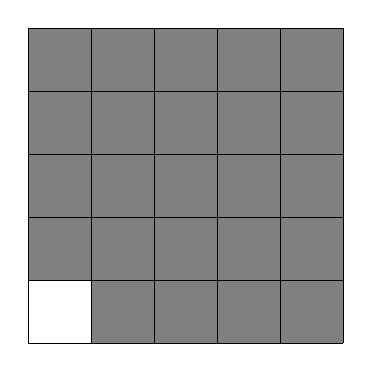
\begin{tikzpicture}[scale=0.8]
        \foreach \x in {0,...,4} {
            \foreach \y in {0,...,4} {
                \fill[gray] (\x,\y) rectangle ++(1,1);
            }
        }
        \fill[white] (0, 0) rectangle ++(1,1);
        \draw[step=1cm,ultra thin,black] (0,0) grid (5,5);
    \end{tikzpicture}
    \caption{\centering Losowe pole startowe.}
    \label{fig:prim_step_2}
\end{figure}